% !TEX encoding = UTF-8 Unicode 
% !TEX root = praca.tex

\subsection{Research scenario 2 results analysis}

The following figures illustrate the aggregated results from the experiments conducted within Research scenario 2 described in Chapter \ref{chap:research_scenarios}.

\begin{figure}[H]
    \begin{minipage}{.48\textwidth}
        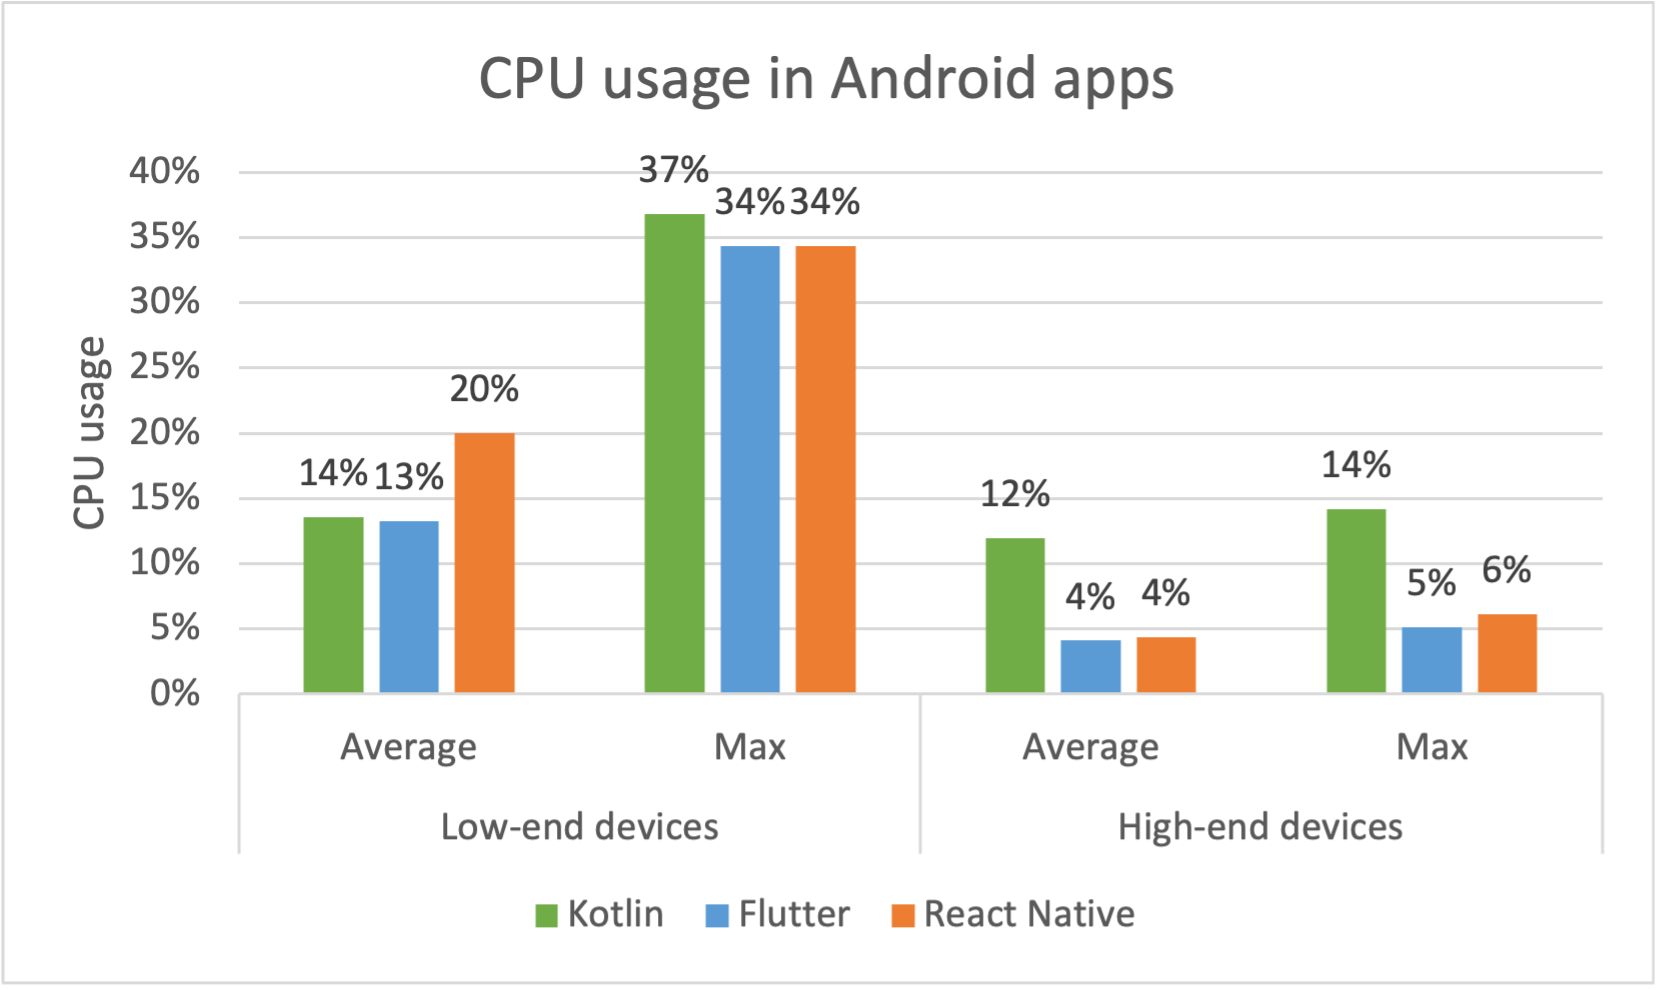
\includegraphics[width=\textwidth]{img/scenario2_cpu_android}
        \caption{Research scenario 2: CPU usage in Android apps (Source: Own work)}
        \label{fig:s2_cpu_android}
    \end{minipage}
    \hfill
    \begin{minipage}{.48\textwidth}
        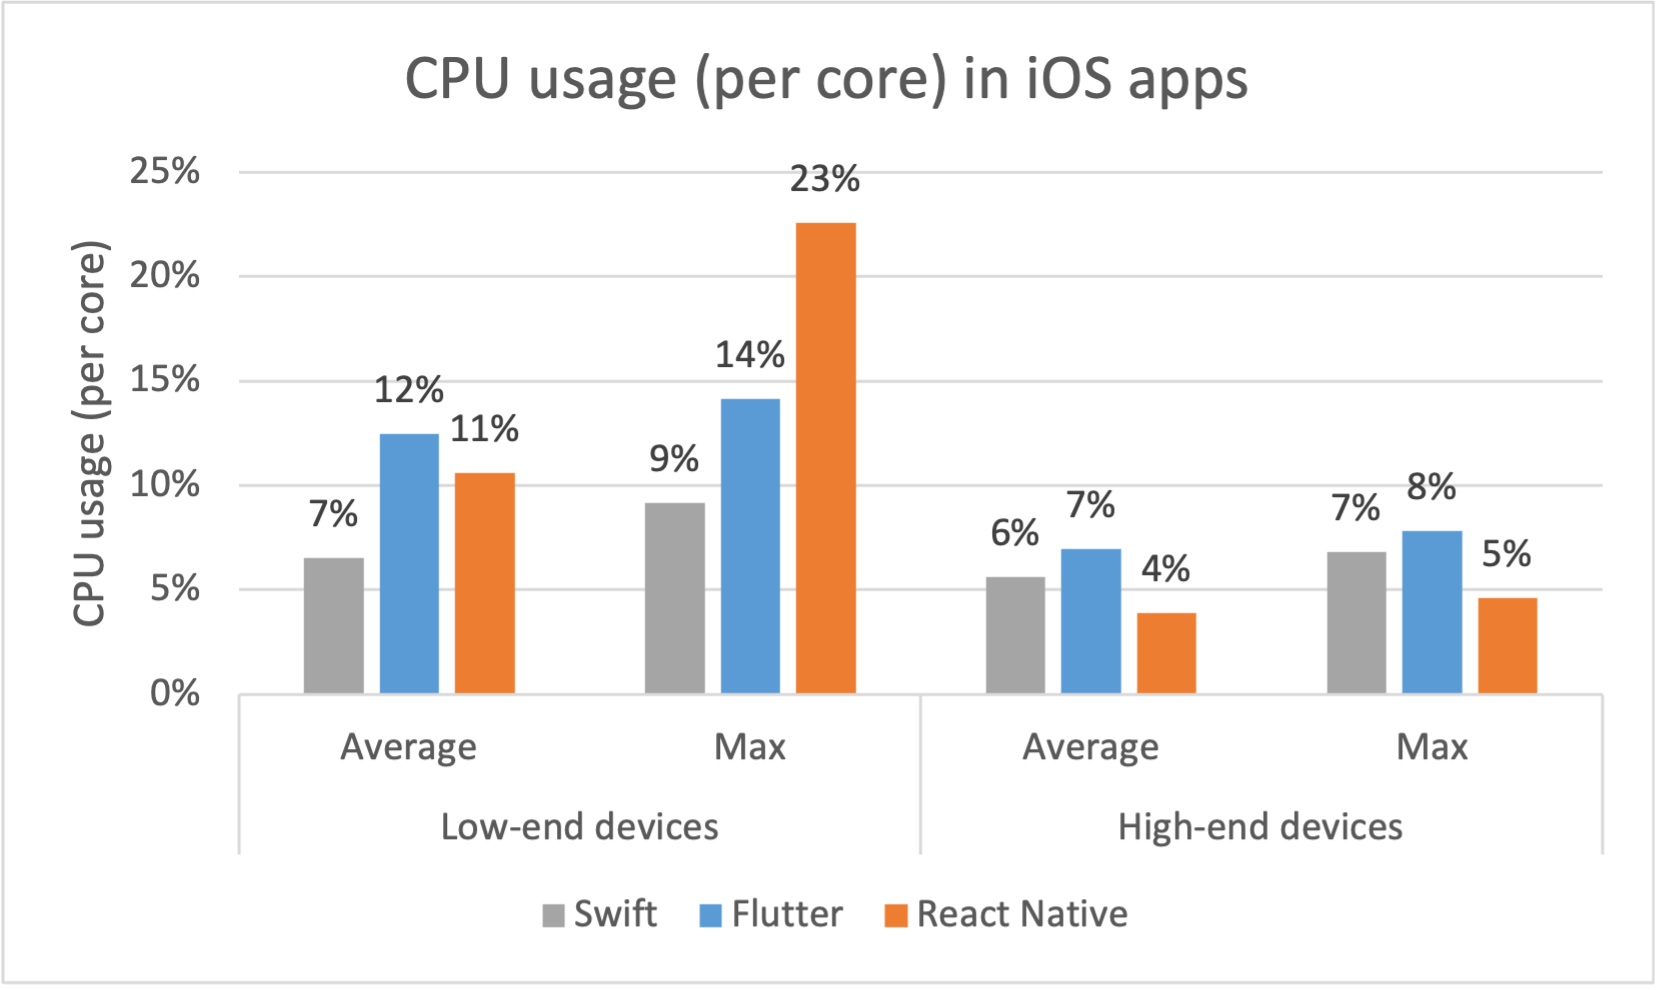
\includegraphics[width=\textwidth]{img/scenario2_cpu_ios}
        \caption{Research scenario 2: CPU usage in iOS apps (Source: Own work)}
        \label{fig:s2_cpu_ios}
    \end{minipage}
\end{figure}

Figures \ref{fig:s2_cpu_android} and \ref{fig:s2_cpu_ios} show the comparison of CPU usage among Android and iOS apps developed with Kotlin, Swift, Flutter, and React Native. In the case of Android apps, on lower-end devices, Kotlin and Flutter apps perform similarly, while React Native apps require slightly more CPU resources. However, on high-end devices, Flutter and React Native apps exhibit very low CPU usage and visibly outperform Kotlin apps. Swift apps running on low-end devices require the least CPU capacity, 7\% on average. Flutter and React Native apps exhibit similar CPU loads; however, the latter experience higher spikes. On high-end devices, all three technologies offer excellent performance while keeping CPU load within the threshold of 4--8\%.

\begin{figure}[H]
    \begin{minipage}{.48\textwidth}
        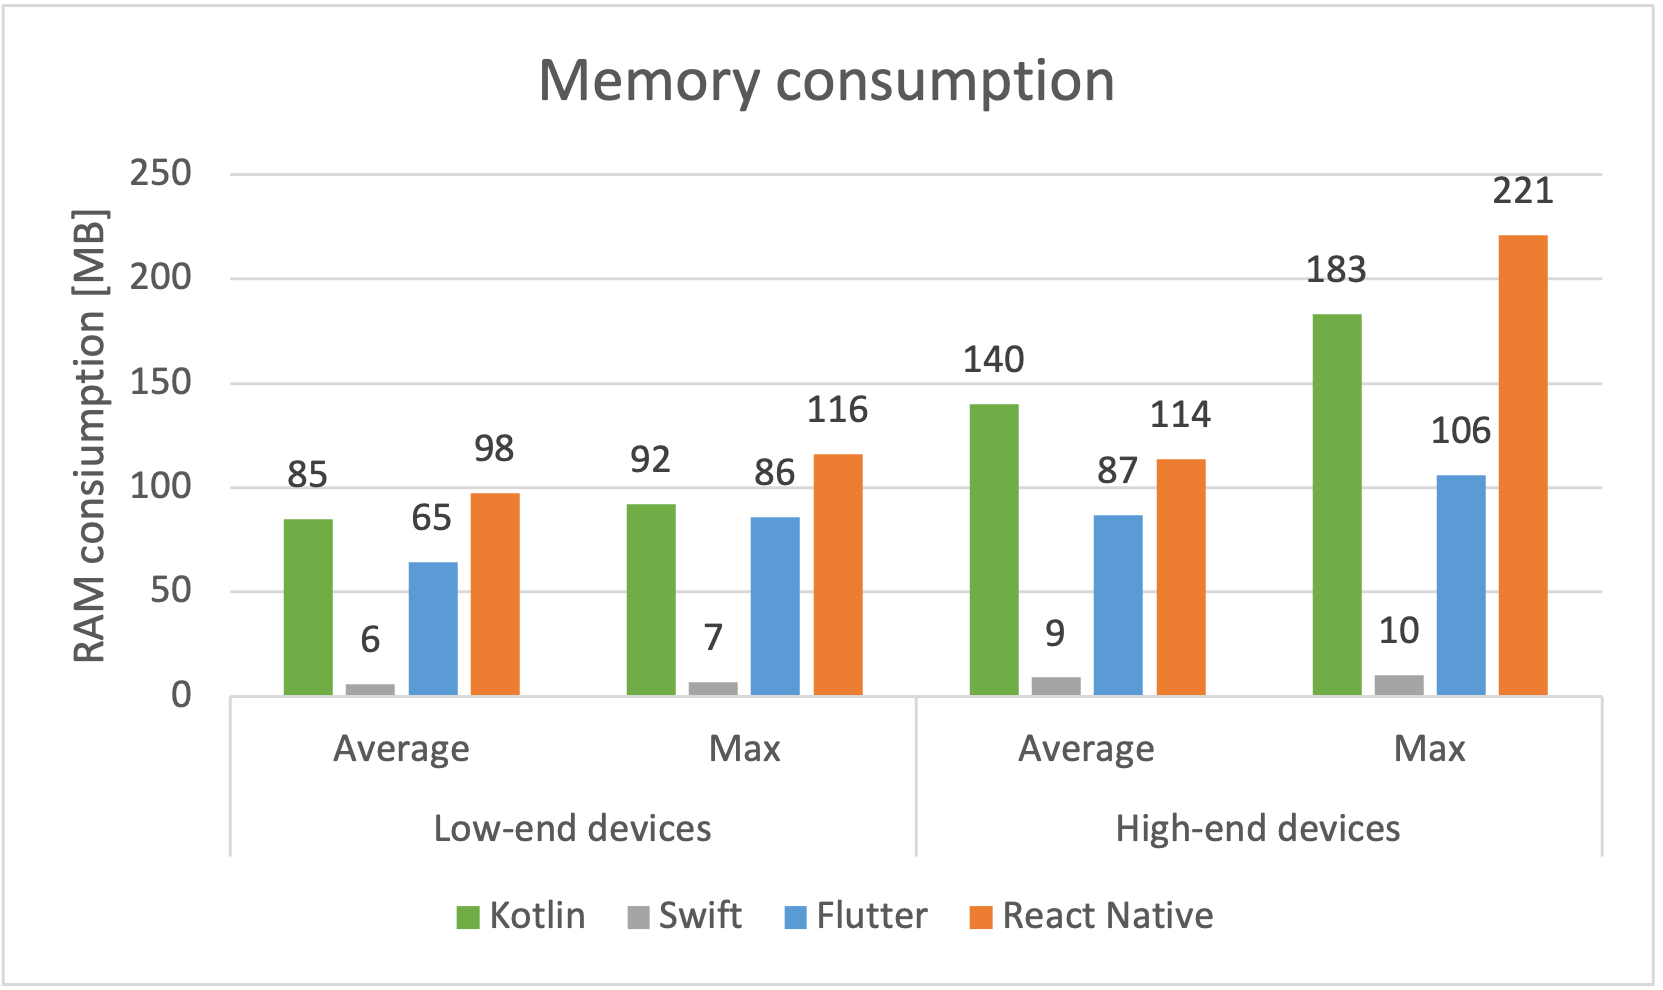
\includegraphics[width=\textwidth]{img/scenario2_ram}
        \caption{Research scenario 2: Memory consumption (Source: Own work)}
        \label{fig:s2_ram}
    \end{minipage}
    \hfill
    \begin{minipage}{.48\textwidth}
        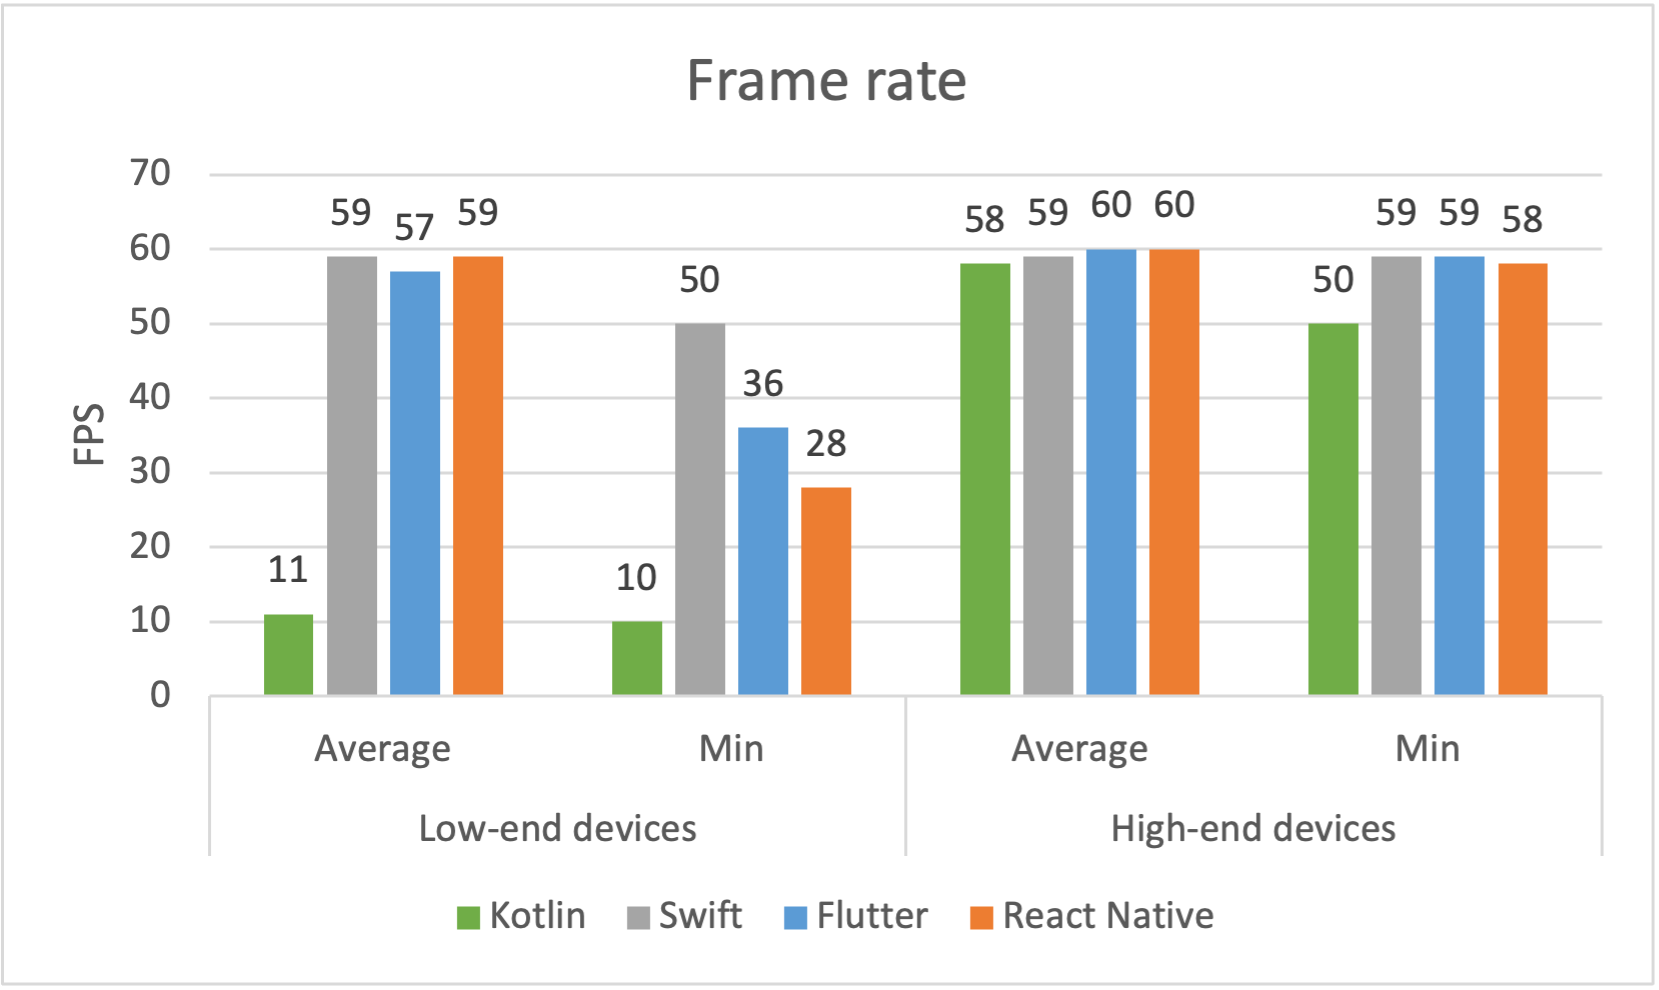
\includegraphics[width=\textwidth]{img/scenario2_fps}
    \caption{Research scenario 2: Frame rate (Source: Own work)}
    \label{fig:s2_fps}
    \end{minipage}
\end{figure}

Figure \ref{fig:s2_ram} shows the comparison of memory consumption among Android and iOS apps developed with Kotlin, Swift, Flutter, and React Native. Swift apps again demonstrate extremely low memory usage compared to other technologies and do not experience any spikes. Flutter apps slightly outperform Kotlin and React Native apps. Kotlin and React Native apps results are rather comparable. The former utilize less memory on low-end devices, and the latter require less memory on high-end devices, although they still experience higher spikes.

\bigskip

Figure \ref{fig:s2_fps} shows the comparison of frame rate among Android and iOS apps developed with Kotlin, Swift, Flutter, and React Native. On high-end devices, each technology exhibits similar performance, maintaining 58--FPS on average. Kotlin apps experience the biggest FPS drops; however, a minimum of 50 FPS is still not a concerning result. On low-end devices, Swift, Flutter, and React Native offer the same great performance, while Kotlin apps seem to suffer from a very low average frame rate of 11\%. Such a result corresponds to users experiencing visible stutters and lags. 

\clearpage
